%%%%%%%%%%%%%%%%%%%%%%%%%%%%%%%%%%%%%%%%%%%%%%%%%%%%%%%%%%%%%%%%%%
%%%%%%%% ICML 2017 EXAMPLE LATEX SUBMISSION FILE %%%%%%%%%%%%%%%%%
%%%%%%%%%%%%%%%%%%%%%%%%%%%%%%%%%%%%%%%%%%%%%%%%%%%%%%%%%%%%%%%%%%

% Use the following line _only_ if you're still using LaTeX 2.09.
%\documentstyle[icml2017,epsf,natbib]{article}
% If you rely on Latex2e packages, like most moden people use this:
\documentclass{article}

% use Times
\usepackage{times}
% For figures
\usepackage{graphicx} % more modern
%\usepackage{epsfig} % less modern
\usepackage{subfigure} 

% For citations
\usepackage{natbib}

% For algorithms
\usepackage{algorithm}
\usepackage{algorithmic}

% As of 2011, we use the hyperref package to produce hyperlinks in the
% resulting PDF.  If this breaks your system, please commend out the
% following usepackage line and replace \usepackage{icml2017} with
% \usepackage[nohyperref]{icml2017} above.
\usepackage{hyperref}

% Packages hyperref and algorithmic misbehave sometimes.  We can fix
% this with the following command.
\newcommand{\theHalgorithm}{\arabic{algorithm}}

% Employ the following version of the ``usepackage'' statement for
% submitting the draft version of the paper for review.  This will set
% the note in the first column to ``Under review.  Do not distribute.''
%\usepackage{icml2017} 

% Employ this version of the ``usepackage'' statement after the paper has
% been accepted, when creating the final version.  This will set the
% note in the first column to ``Proceedings of the...''
\usepackage[accepted]{icml2017}


% The \icmltitle you define below is probably too long as a header.
% Therefore, a short form for the running title is supplied here:
% \icmltitlerunning{Submission and Formatting Instructions for ICML 2017}

\begin{document} 

\twocolumn[
\icmltitle{Assignment 1}

% It is OKAY to include author information, even for blind
% submissions: the style file will automatically remove it for you
% unless you've provided the [accepted] option to the icml2017
% package.

% list of affiliations. the first argument should be a (short)
% identifier you will use later to specify author affiliations
% Academic affiliations should list Department, University, City, Region, Country
% Industry affiliations should list Company, City, Region, Country

% you can specify symbols, otherwise they are numbered in order
% ideally, you should not use this facility. affiliations will be numbered
% in order of appearance and this is the preferred way.
% \icmlsetsymbol{equal}{*}

\begin{icmlauthorlist}
\icmlauthor{V Nidhin Krishnan}{iisc}

\end{icmlauthorlist}

\icmlaffiliation{iisc}{Indian Institute of Science, Bangalore}

\icmlcorrespondingauthor{V Nidhin Krishnan}{nidhinkrishnanv@gmail.com}

% You may provide any keywords that you 
% find helpful for describing your paper; these are used to populate 
% the "keywords" metadata in the PDF but will not be shown in the document
\icmlkeywords{boring formatting information, machine learning, ICML}

\vskip 0.3in
]

% this must go after the closing bracket ] following \twocolumn[ ...

% This command actually creates the footnote in the first column
% listing the affiliations and the copyright notice.
% The command takes one argument, which is text to display at the start of the footnote.
% The \icmlEqualContribution command is standard text for equal contribution.
% Remove it (just {}) if you do not need this facility.

\printAffiliationsAndNotice{}  % leave blank if no need to mention equal contribution
% \printAffiliationsAndNotice{\icmlEqualContribution} % otherwise use the standard text.

% \begin{abstract} 
% Assignment submission for ML with Large Dataset. Implemented code for local and hadoop version of Naive Bayes. 
% \end{abstract} 

\section{Model Description}
There are two pass of map reduce for both train and test. One more map reduce pass is used to create a cache to be shared by all reducers. The cache is of size 3.5KB. For training in the first pass event counts like "Y=label X=word	22" are produced. In the next pass the output is such that the key is a word and values are count of word for a particular label. This output and test data are used as input for testing. In the first pass the output has the key as label of data and values as words and its counts. Then this output and test data are used to predict the labels of the test data. The final output is the id and its predicted labels, number of correct predictions and total number of data.

\section{Code}
The code is uploaded at https://github.com/nidhinkrishnanv/Naive-Bayes-classifier. Referred \cite{website} for starter code for using python with hadoop .


\section{Accuracy}
\begin{center}
\begin{tabular}{ lll} 
 \hline
 \abovespace\belowspace
  &  Development(\%) & Test(\%)  \\ 
 \hline
  \abovespace
 local & 98.25 & 98.31 \\ 
 \belowspace
 hadoop & 73.44 & 77.01 \\ 
 \hline
\end{tabular}
\end{center}


\section{Run time}

\begin{center}
\begin{tabular}{ lll } 
 \hline
\abovespace\belowspace
  & Train(sec) & Test(sec)  \\ 
 \hline
 \abovespace
 local & 18.45 & 78.96 \\ 
 hadoop(10) & 106 & 46 \\
 \belowspace
 hadoop(1) & 196 & 181 \\ 
 \hline
\end{tabular}
\end{center}

Runtime for local and hadoop run of map reduce. In the table hadoop(10) is the run time for 10 Reducers and hadoop(1) for 1 Reducer.

\begin{figure}
\vskip 0.2in
\centerline{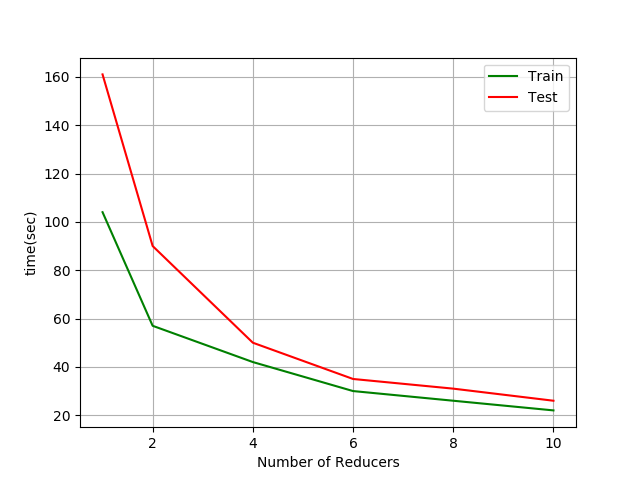
\includegraphics[width=\linewidth]{graph.png}}
\caption{Run time for number of reducers from 2 to 10}
\label{fig-graph}
\vskip -0.2in
\end{figure}

When using 2 and 4 reducer there is exponential decrease in time. Then it starts to flatten out at 8 to 10. Which can be see in  Figure~\ref{fig-graph}.


\section{Number of parameters}
\begin{center}
\begin{tabular}{ ll } 
 \hline
 \abovespace\belowspace
  & Parametes  \\ 
\hline
\abovespace
 local & 1317112 \\ 
\belowspace
 hadoop & 2230872 \\ 
 \hline
\end{tabular}
\end{center}



% In the unusual situation where you want a paper to appear in the
% references without citing it in the main text, use \nocite
\nocite{website}

\bibliography{example_paper}
\bibliographystyle{icml2017}

\end{document} 


% This document was modified from the file originally made available by
% Pat Langley and Andrea Danyluk for ICML-2K. This version was
% created by Lise Getoor and Tobias Scheffer, it was slightly modified  
% from the 2010 version by Thorsten Joachims & Johannes Fuernkranz, 
% slightly modified from the 2009 version by Kiri Wagstaff and 
% Sam Roweis's 2008 version, which is slightly modified from 
% Prasad Tadepalli's 2007 version which is a lightly 
% changed version of the previous year's version by Andrew Moore, 
% which was in turn edited from those of Kristian Kersting and 
% Codrina Lauth. Alex Smola contributed to the algorithmic style files.  
